\begin{Large}
\vskip1cm
\begin{figure}[h]
	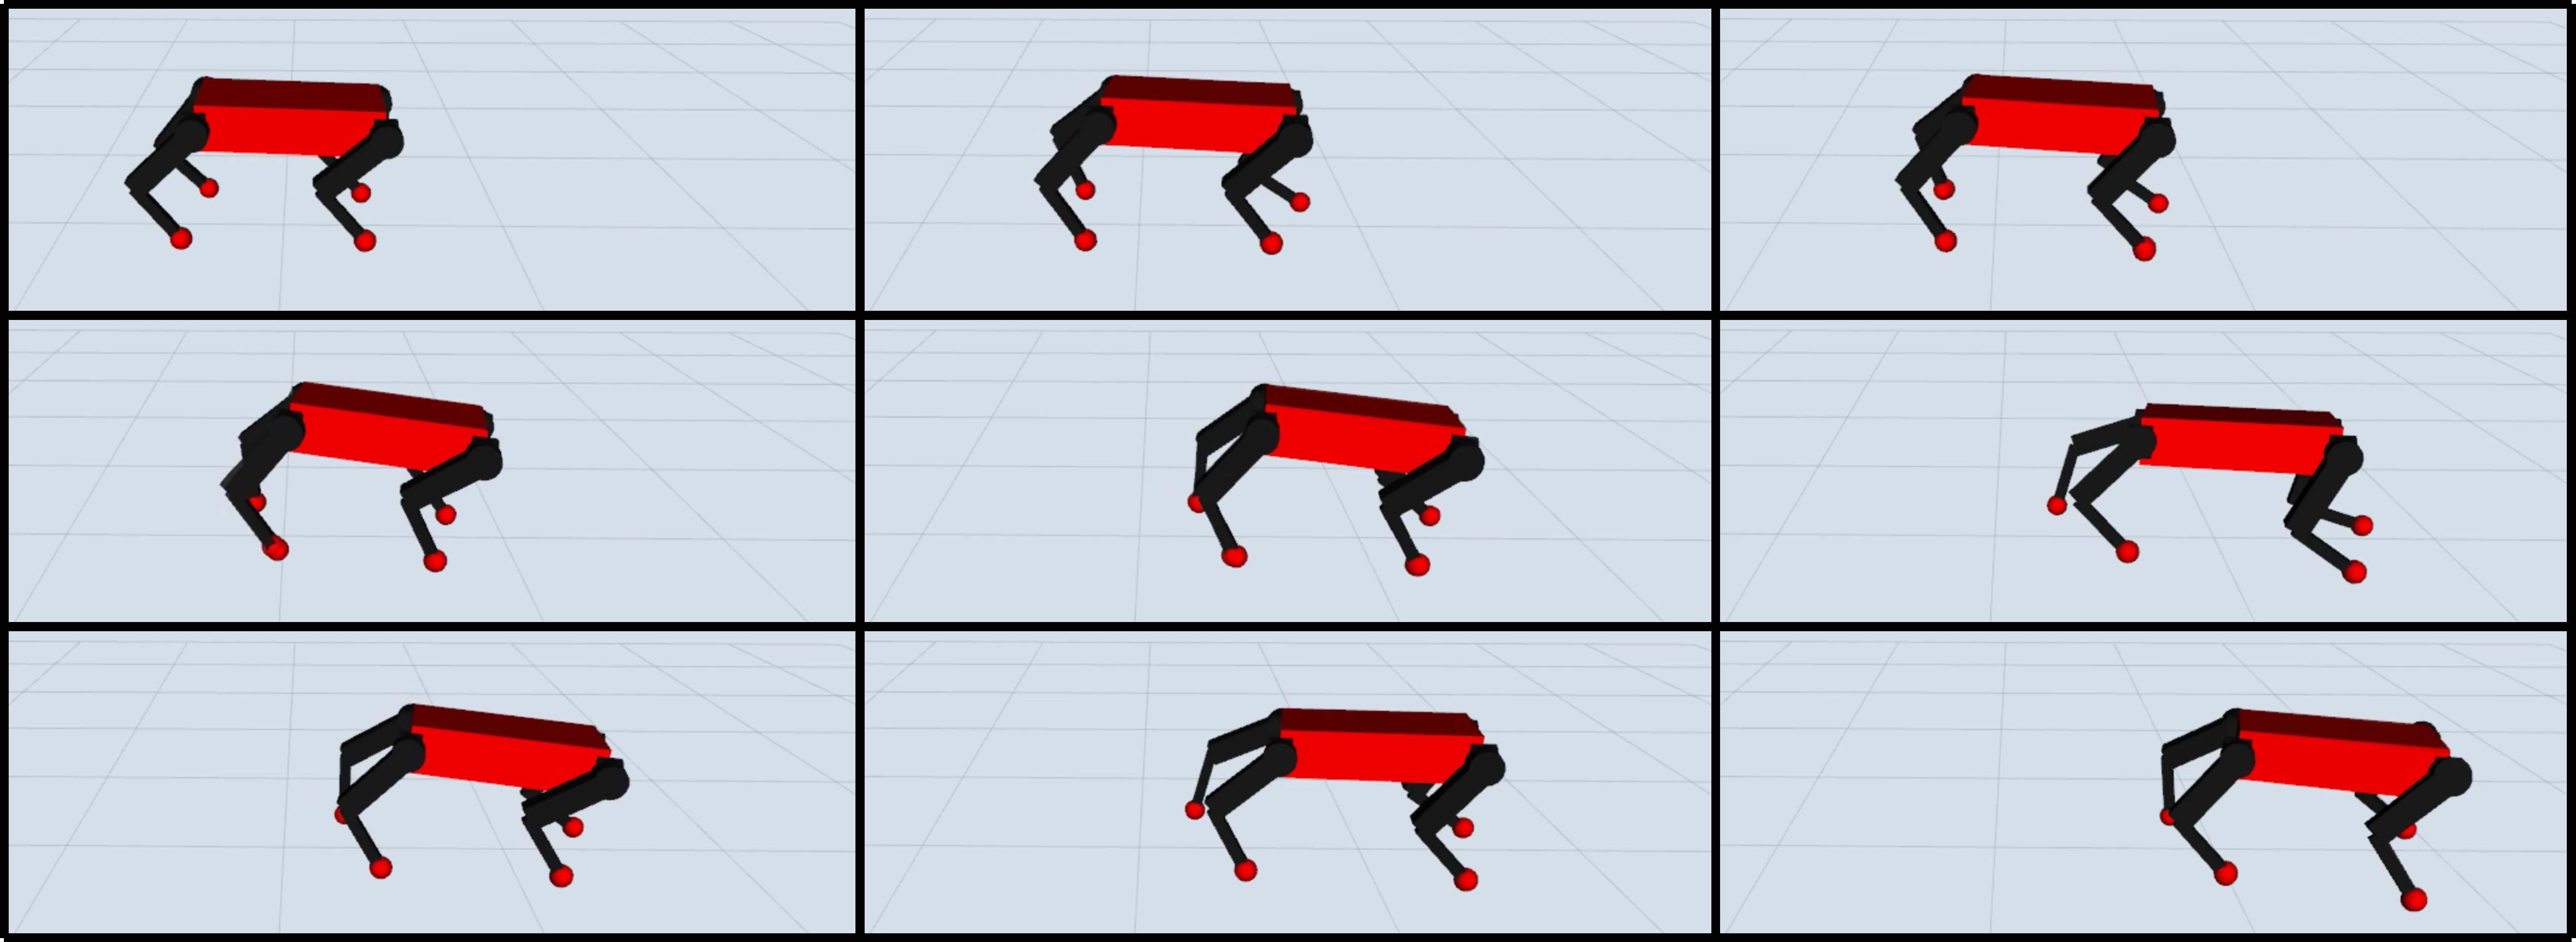
\includegraphics[width=0.8\textwidth]{docs/imgs/proof_of_concept.pdf}
\end{figure}
{\Large We designed a proof of concept example to test the use of the framework. Focus on quadruped locomotion, with the RL agent in charge of RHC twist commands + stepping phases selection. Agent exposed to proprioceptive measurements (orientation, meas twist, refs, rhc running cost/ constraint violation, stepping phases). We use a custom implementation of PPO which correctly differentiates between terminations and truncations. RHC developed in HHCM, not open for now. Random walk on flat ground. Twist reference tracking. Describe the training env: what the agent sees, configurations, etc....}
\end{Large}

	